\documentclass[14pt]{extbook}
\usepackage{multicol, enumerate, enumitem, hyperref, color, soul, setspace, parskip, fancyhdr} %General Packages
\usepackage{amssymb, amsthm, amsmath, bbm, latexsym, units, mathtools} %Math Packages
\everymath{\displaystyle} %All math in Display Style
% Packages with additional options
\usepackage[headsep=0.5cm,headheight=12pt, left=1 in,right= 1 in,top= 1 in,bottom= 1 in]{geometry}
\usepackage[usenames,dvipsnames]{xcolor}
\usepackage{dashrule}  % Package to use the command below to create lines between items
\newcommand{\litem}[1]{\item#1\hspace*{-1cm}\rule{\textwidth}{0.4pt}}
\pagestyle{fancy}
\lhead{Progress Quiz 4}
\chead{}
\rhead{Version B}
\lfoot{9187-5854}
\cfoot{}
\rfoot{Spring 2021}
\begin{document}

\begin{enumerate}
\litem{
Which of the following equations \textit{could} be of the graph presented below?
\begin{center}
    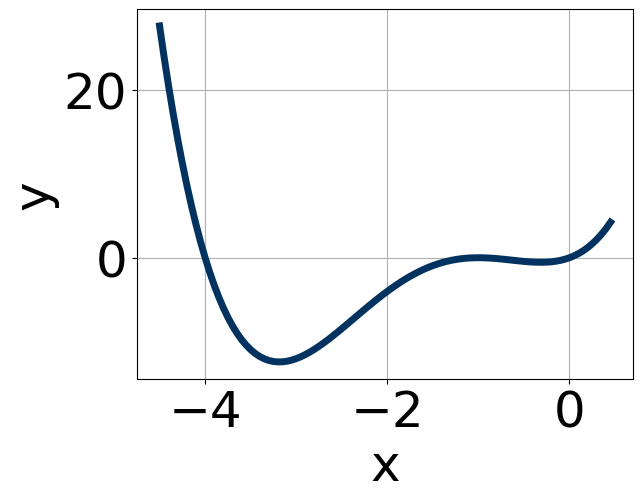
\includegraphics[width=0.5\textwidth]{../Figures/polyGraphToFunctionCopyB.png}
\end{center}
\begin{enumerate}[label=\Alph*.]
\item \( 19x^{5} (x + 1)^{10} (x + 4)^{9} \)
\item \( -12x^{11} (x + 1)^{4} (x + 4)^{11} \)
\item \( 13x^{5} (x + 1)^{6} (x + 4)^{4} \)
\item \( 5x^{7} (x + 1)^{11} (x + 4)^{4} \)
\item \( -2x^{8} (x + 1)^{10} (x + 4)^{11} \)

\end{enumerate} }
\litem{
Describe the end behavior of the polynomial below.\[ f(x) = -9(x + 4)^{5}(x - 4)^{6}(x + 3)^{2}(x - 3)^{3} \]\begin{enumerate}[label=\Alph*.]
\begin{multicols}{2}\item 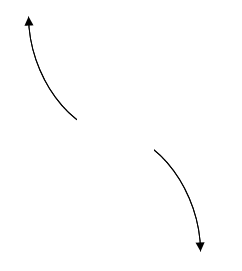
\includegraphics[width = 0.3\textwidth]{../Figures/polyEndBehaviorCopyAB.png}\item 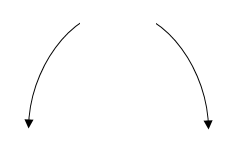
\includegraphics[width = 0.3\textwidth]{../Figures/polyEndBehaviorCopyBB.png}\item 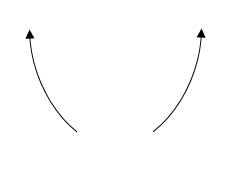
\includegraphics[width = 0.3\textwidth]{../Figures/polyEndBehaviorCopyCB.png}\item 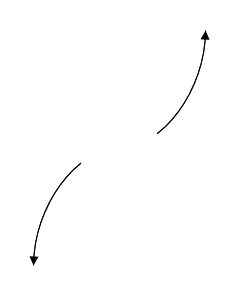
\includegraphics[width = 0.3\textwidth]{../Figures/polyEndBehaviorCopyDB.png}\end{multicols}\item None of the above.
\end{enumerate} }
\litem{
Construct the lowest-degree polynomial given the zeros below. Then, choose the intervals that contain the coefficients of the polynomial in the form $ax^3+bx^2+cx+d$.\[ \frac{-4}{3}, -3, \text{ and } \frac{-6}{5} \]\begin{enumerate}[label=\Alph*.]
\item \( a \in [9, 22], b \in [42, 48], c \in [-30, -28], \text{ and } d \in [-76, -66] \)
\item \( a \in [9, 22], b \in [81, 91], c \in [136, 139], \text{ and } d \in [-76, -66] \)
\item \( a \in [9, 22], b \in [81, 91], c \in [136, 139], \text{ and } d \in [71, 75] \)
\item \( a \in [9, 22], b \in [-85, -80], c \in [136, 139], \text{ and } d \in [-76, -66] \)
\item \( a \in [9, 22], b \in [-51, -46], c \in [-18, -13], \text{ and } d \in [71, 75] \)

\end{enumerate} }
\litem{
Describe the zero behavior of the zero $x = -2$ of the polynomial below.\[ f(x) = 5(x - 2)^{9}(x + 2)^{14}(x + 6)^{2}(x - 6)^{3} \]\begin{enumerate}[label=\Alph*.]
\begin{multicols}{2}\item 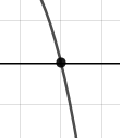
\includegraphics[width = 0.3\textwidth]{../Figures/polyZeroBehaviorAB.png}\item 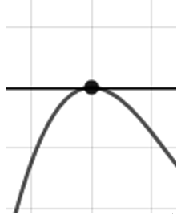
\includegraphics[width = 0.3\textwidth]{../Figures/polyZeroBehaviorBB.png}\item 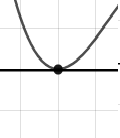
\includegraphics[width = 0.3\textwidth]{../Figures/polyZeroBehaviorCB.png}\item 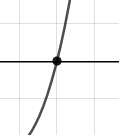
\includegraphics[width = 0.3\textwidth]{../Figures/polyZeroBehaviorDB.png}\end{multicols}\item None of the above.
\end{enumerate} }
\litem{
Describe the end behavior of the polynomial below.\[ f(x) = -6(x - 6)^{5}(x + 6)^{6}(x - 8)^{2}(x + 8)^{3} \]\begin{enumerate}[label=\Alph*.]
\begin{multicols}{2}\item 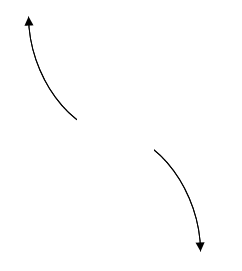
\includegraphics[width = 0.3\textwidth]{../Figures/polyEndBehaviorAB.png}\item 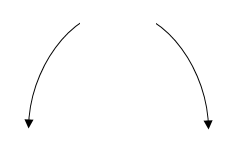
\includegraphics[width = 0.3\textwidth]{../Figures/polyEndBehaviorBB.png}\item 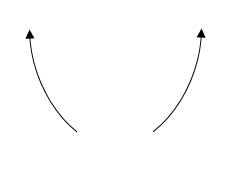
\includegraphics[width = 0.3\textwidth]{../Figures/polyEndBehaviorCB.png}\item 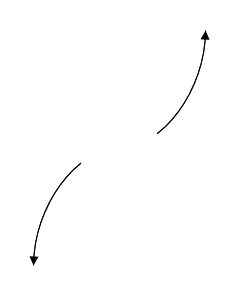
\includegraphics[width = 0.3\textwidth]{../Figures/polyEndBehaviorDB.png}\end{multicols}\item None of the above.
\end{enumerate} }
\litem{
Construct the lowest-degree polynomial given the zeros below. Then, choose the intervals that contain the coefficients of the polynomial in the form $x^3+bx^2+cx+d$.\[ -3 - 2 i \text{ and } -1 \]\begin{enumerate}[label=\Alph*.]
\item \( b \in [-0.9, 1.1], c \in [3.8, 5.6], \text{ and } d \in [2.51, 3.71] \)
\item \( b \in [-0.9, 1.1], c \in [2.8, 3.5], \text{ and } d \in [1.06, 2.89] \)
\item \( b \in [5.9, 10.8], c \in [17.6, 19.4], \text{ and } d \in [12.15, 13.95] \)
\item \( b \in [-8, -3.3], c \in [17.6, 19.4], \text{ and } d \in [-13.5, -12.06] \)
\item \( \text{None of the above.} \)

\end{enumerate} }
\litem{
Which of the following equations \textit{could} be of the graph presented below?
\begin{center}
    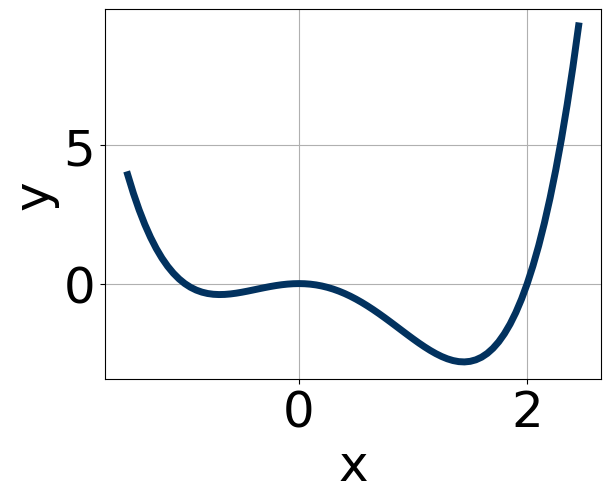
\includegraphics[width=0.5\textwidth]{../Figures/polyGraphToFunctionB.png}
\end{center}
\begin{enumerate}[label=\Alph*.]
\item \( -12x^{4} (x + 4)^{10} (x - 2)^{11} \)
\item \( 15x^{8} (x + 4)^{11} (x - 2)^{11} \)
\item \( -15x^{6} (x + 4)^{11} (x - 2)^{7} \)
\item \( 17x^{11} (x + 4)^{7} (x - 2)^{7} \)
\item \( -17x^{9} (x + 4)^{7} (x - 2)^{11} \)

\end{enumerate} }
\litem{
Construct the lowest-degree polynomial given the zeros below. Then, choose the intervals that contain the coefficients of the polynomial in the form $x^3+bx^2+cx+d$.\[ 5 + 2 i \text{ and } -3 \]\begin{enumerate}[label=\Alph*.]
\item \( b \in [5, 11], c \in [-1.05, -0.7], \text{ and } d \in [-96, -81] \)
\item \( b \in [-13, -2], c \in [-1.05, -0.7], \text{ and } d \in [87, 93] \)
\item \( b \in [-2, 5], c \in [-2.32, -1.02], \text{ and } d \in [-17, -12] \)
\item \( b \in [-2, 5], c \in [0.87, 1.64], \text{ and } d \in [-6, -1] \)
\item \( \text{None of the above.} \)

\end{enumerate} }
\litem{
Describe the zero behavior of the zero $x = 3$ of the polynomial below.\[ f(x) = -8(x + 3)^{8}(x - 3)^{13}(x - 7)^{3}(x + 7)^{7} \]\begin{enumerate}[label=\Alph*.]
\begin{multicols}{2}\item 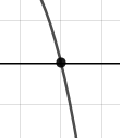
\includegraphics[width = 0.3\textwidth]{../Figures/polyZeroBehaviorCopyAB.png}\item 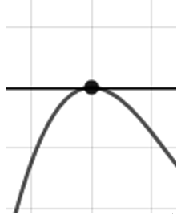
\includegraphics[width = 0.3\textwidth]{../Figures/polyZeroBehaviorCopyBB.png}\item 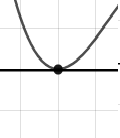
\includegraphics[width = 0.3\textwidth]{../Figures/polyZeroBehaviorCopyCB.png}\item 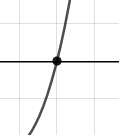
\includegraphics[width = 0.3\textwidth]{../Figures/polyZeroBehaviorCopyDB.png}\end{multicols}\item None of the above.
\end{enumerate} }
\litem{
Construct the lowest-degree polynomial given the zeros below. Then, choose the intervals that contain the coefficients of the polynomial in the form $ax^3+bx^2+cx+d$.\[ \frac{6}{5}, \frac{2}{3}, \text{ and } \frac{-1}{5} \]\begin{enumerate}[label=\Alph*.]
\item \( a \in [70, 76], b \in [-125, -119], c \in [32, 39], \text{ and } d \in [-13, 1] \)
\item \( a \in [70, 76], b \in [125, 126], c \in [32, 39], \text{ and } d \in [-13, 1] \)
\item \( a \in [70, 76], b \in [53, 60], c \in [-59, -48], \text{ and } d \in [-13, 1] \)
\item \( a \in [70, 76], b \in [-125, -119], c \in [32, 39], \text{ and } d \in [11, 16] \)
\item \( a \in [70, 76], b \in [154, 164], c \in [88, 90], \text{ and } d \in [11, 16] \)

\end{enumerate} }
\end{enumerate}

\end{document}